\section{性能}
\label{secPerformance}

在本节中,将在几个突出的不同的特性条件下比较控制器。 
如前所述,对于小的误差,所有的控制器的行为都类似(并且设置 $\gainAtt=\diag{\gainAttRed,\gainAttRed,\gainAttYaw}$)。
然而,对于大的姿态误差,会出现显著的差异。
具体来说,它将显示,斜对称控制器将在任意持续时间内保持几乎是 180$^\circ$ 的姿态误差;在安全关键环境中部署时,这是一个特别值得关注的问题。

在每种情况下,基于旋转向量的控制器在总的姿态误差方面表现最好;并且具体而言,基于旋转向量的控制器似乎比斜对称控制更可取。
然而,当仅考虑推力方向误差时,倾斜优先控制器(包括基于四元数的控制器以及拟议的控制器)的性能优于旋转向量控制器。
此外,拟议的控制器将被证明优于基于四元数的控制器。

\subsection{共用模拟参数}
对于所有仿真,姿态控制参数如下:
\begin{align}
	\gainAtt    &= \diag{\gainAttRed,\gainAttRed,\gainAttYaw}
\\  \gainAttRed &= 4 \ \mathrm{s}^{-2}
\\  \gainAttYaw &= 1 \ \mathrm{s}^{-2}
\\  \gainRates  &= \sqrt{2}\;\diag{2, 2, 1} \ \mathrm{s}^{-1}
\end{align}
因此,所有的控制器在一阶上表现为质量-弹簧-阻尼器,其倾斜方向的自然频率为 $2$rad/s,并且偏航方向为 $1$rad/s,以及阻尼比为 $\sqrt{1/2}\approx0.707$。
所有控制器在实验中共享相同的控制参数。

\subsection{斜对称控制器的任意缓慢收敛}
\label{secPerfInitAngVel}

\begin{figure}
  \centering
  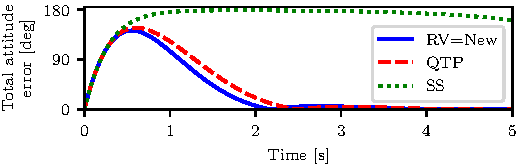
\includegraphics{Figures/fig_case1.pdf}
  \caption{
  来自 \secref{secPerfInitAngVel} 的示例:从大的初始角速度恢复,显示了斜对称控制器的灾难性性能。 
  	`SS' 指的是斜对称控制器方程 \eqref{eqDefInputSS},`RV' 指的是旋转向量控制器方程 \eqref{eqDefInputRotVec},`QTP' 指的是基于四元数的倾斜优先级控制器方程 \eqref{eqDefInputQTP},并且 `New' 指的是提议的控制器方程 \eqref{eqDefInputNew}。
  	基于旋转向量的控制器的行为与新控制器的行为相同。
  }
  \label{figCaseLargeInitVel}
\end{figure}


假设飞行器静止起步,但有一个姿态误差为 $\rho\approx180^\circ$。
从方程 \eqref{eqSkewSymmControllerAxAngle} 可以清楚地看出,由于采用了角度的正弦,斜对称控制器指令的角加速度大约为零。
在飞行中,这本身就是一个安全问题 -- 虽然只要姿态不精确在 $\rho=180^\circ$ 处,最终会收敛到所需的姿态,但这可能需要任意长的时间。
具体而言,当姿态误差超过 $90^\circ$ 时,姿态控制的`刚度'开始\emph{下降}。
在四个控制器中,这是斜对称控制器所独有的。 

为了更生动地说明这一潜在的安全问题,考虑一个初始姿态误差为零的飞行器,但角速度为 $\angVel(0)=\mrb{10.8,0,0}$rad/s。
系统的反应显示在 \figref{figCaseLargeInitVel}。
值得注意的是,所有控制器都能迅速将角速度降为零,但斜对称控制器的姿态误差徘徊在 180$^\circ$ 左右。
基于旋转向量的控制器和所提出的新控制器性能相同,并且略优于基于四元数的推力优先控制器。 

尽管之前已经注意到斜对称控制器收敛缓慢的可能性 \cite{lee2012exponential},但该控制器在文献中仍然很受欢迎(例如文献 \cite{simha2017almost,sreenath2013geometric,rashad2017design})。

\subsection{倾斜优先的优点}
\label{secPerfAdvantageTiltPrior}
\begin{figure}
  \centering
  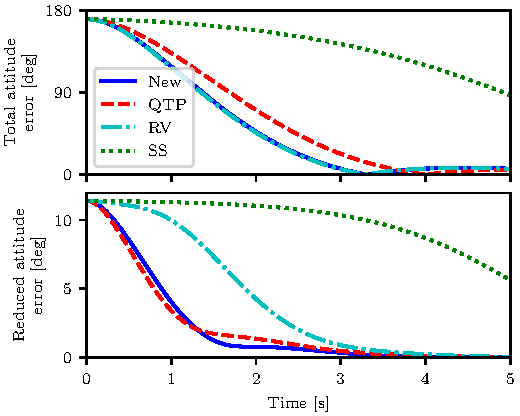
\includegraphics{Figures/fig_case2.pdf}
  \caption{
  来自 \secref{secPerfAdvantageTiltPrior} 的示例:从大的初始偏航误差中恢复,初始倾斜误差较小,显示了拟议的控制器的推力方向的更快速收敛。
  }
  \label{figCaseLargeLargeYaw}
\end{figure}

根据设计,倾斜优先控制器应使飞行器的推力方向更快地收敛到期望的推力方向。
作为这种行为的一个示例,考虑一个从静止开始的飞行器,但围绕轴 $\rotAxis(0)\approx\mrb{0.0995,0,0.995}$ 已旋转 170$^\circ$,因此飞行器有很大的偏航误差,但只有轻微的倾斜误差。
在 \figref{figCaseLargeLargeYaw} 中比较了控制器的性能,可以看出,基于四元数的控制器和拟议的控制器都比基于旋转向量的控制器减少倾斜误差的速度更快得多。
此外,在这种特定情况下,对于总的姿态误差,拟议的控制器的性能实际上与基于旋转向量的控制器没有什么区别,而基于四元数的倾斜优先控制器的性能明显较差。

斜对称控制器的性能再次特别差。
注意,从某种意义上说,这是一个比上一个例子更``友好''的初始条件,因为飞行器现在主要有一个初始偏航误差,理想情况下,这对飞行器的动力学影响应该很小。
此外,由于多旋翼飞机典型的视觉旋转对称性,这种错误在起飞时比较典型(例如,如果操作员错误地放置飞行器)。
此外,偏航误差没有被特别仔细地选择;对于 $10/180\approx5\%$ 的偏航范围,性能不会比图中所示的更好。

\subsection{倾斜优先的缺点}
\label{secPerfDisadvantageTiltPrior}
\begin{figure}
  \centering
  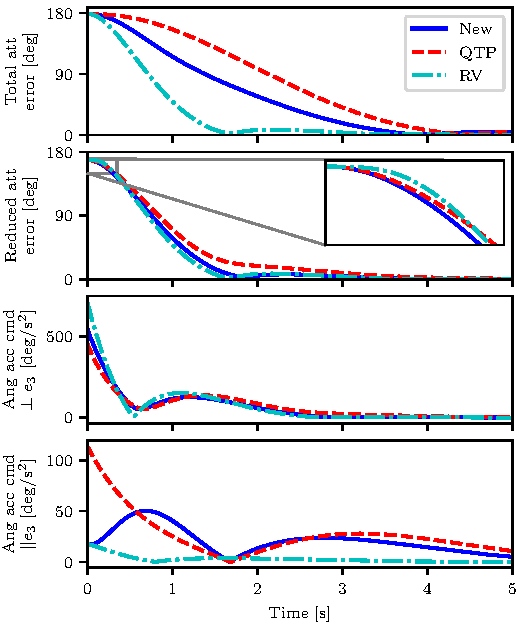
\includegraphics{Figures/fig_case3.pdf}
  \caption{
  来自 \secref{secPerfDisadvantageTiltPrior} 的示例:从大的初始倾斜误差中恢复,初始偏航误差小,显示了基于旋转向量的控制优于拟议的推力优先控制器的例子。
  从上到下:总的姿态误差 $\rotAngle$;减小的姿态误差 $\rotAngleReduced$;垂直于推力方向 $\thrustDir$ 的指令角加速度分量的量值;以及平行于推力方向的指令角加速度分量的量值。
  	插图显示了减小的姿态反应的细节。
  }
  \label{figCaseLargeLargeTilt}
\end{figure}

对于总的姿态误差(而不仅仅是倾斜误差),基于旋转向量的控制通常会优于拟议的控制器,因为它仅直接作用于该误差。
例如,考虑一个围绕轴 $\rotAxis(0)\approx\mrb{0.995,0,0.0995}$的 179$^\circ$ 的初始旋转。
围绕垂直于飞行器推力方向的任意轴线进行的旋转将使飞行器的倾斜误差近乎为零,然而,通过改变旋转轴线的选择,剩余的偏航误差可以是零,也可以大到 $180^\circ$。 

在 \figref{figCaseLargeLargeTilt} 中比较了控制器的性能。
正如预期的那样,基于旋转向量的控制在考虑整体姿态误差时表现最好,在这种情况下,倾斜误差也最终收敛得最快。
基于四元数的控制器和新拟议的倾斜优先控制器在整体姿态误差方面的表现都比较差,但在倾斜角度方面,进行初始化时确实优于基于旋转向量的控制器。
值得注意的是,在初始化阶段,拟议的控制器可以最快地减少`减小的姿态误差'。 

此外,值得注意的是,拟议的控制器在倾斜误差和总的角度误差方面都优于基于四元数的控制器。
此外,它在这样做的同时,还指令降低围绕飞行器推力轴的角加速度峰值,如 \figref{figCaseLargeLargeTilt} 底部所示,尽管总的姿态误差下降得更快。
这种特性在多旋翼飞行器中通常是可取的,因为它们能够围绕 $\baseVec{1}$ 和 $\baseVec{2}$ 产生比推力方向 $\baseVec{3}$ 更大的扭矩,而围绕 $\baseVec{3}$ 的大的角加速度指令可能会迅速导致电机推力的饱和。 



